\documentclass[a4paper,12pt]{article}
\usepackage[hidelinks]{hyperref}
\usepackage{graphicx}
\usepackage{float}
\usepackage{caption}
\begin{document}
\begin{center}

%Cover page
\Huge\textbf{Functional Requirements(uWatch digital forensic tool)\\}
																											
\vspace{2 cm}

\LARGE\textbf{Group Name:} MPHETamines\newline
 
 
\LARGE\textbf{Version:} 1.2\newline
 
 
 
\vspace{0.5 cm}
\begin{tabular}{lr}
Taariq Ghoord&10132806
\\ 
Martha Mohlala&10353403
\\
Phethile Mkhabela&12097561
\\
Sboniso Masilela&10416260
\\
Harrison Maphuti Setati&12310043\\
\end{tabular}

\vspace{1cm}
\textbf{Git repository link:\\}
\url{https://github.com/MPHETamines/MPHETamines/}

\vspace{1cm}
\textbf{Date:} 20 May 2015
\end{center}
\pagenumbering{gobble}
\newpage

%table of contents
\tableofcontents







\newpage
\pagenumbering{arabic}

\section{Introduction}
This document sets out the Software Requirements Specification and Technology Neutral Process Design for the COS 301 group project entitled \textit{Online Neighbourhood Watch(ONW aka uWatch)}.
The aim for this project is to follow agile software development approach within which the application functionality is developed 
iteratively. 
The information provided in this document is presented in such a way as to provide precise and testable requirements. The emphasis is on performing an upfront software 
architecture engineering for iterative stimulation of the detailed requirements for a use case so that each use case can be built, tested and deployed before the detailed 
requirements for the next case are added.
\subsection{Project Background}
Crime is a prominent issue in South Africa as it is all over the world, Many criminal activities go unresolved or even attended to due to the lack of evidence or concrete witnesses.  Mobile applications have become increasingly popular all over the world and are used in our everyday and work life for common things such as checking the weather; maps for directions and news feed updates.  Digital forensic science hopes to utilise this increasing growth in the use of mobile applications to address the lack of evidence to crime cases in South Africa.
The application is referred to as Online Neighbourhood Watch(ONW) accessible via mobile devices and computers over the internet.  The two main users of the ONW model are the uploader (user of the mobile device) and the forensic investigator or law enforcement agent. 
This tool is to be used by the citizens of South Africa to capture, collect and store potential evidence which can later be viewed and analysed by the Police department and used in the prosecution and detention of criminals.
\subsection{Project Purpose}
The Online Neighbourhood Watch is aimed to provide a tool that can assist the South African Police Services(SAPS) reduce crime by enabling the members of the community to be part of the judicial system.  The ONW application captures and stores potential digital evidence of criminal activities which will then be accessed by law enforcement agents and digital forensic investigators.  The goal is to enhance the successful rate of trials and secure a higher number of convictions.
The application can be used in various scenarios, basically it should be used in any setting where a community member feels like a crime has been committed, it is then up to the ONW model to decide if the uploaded data is a potential crime scene. The application should enable a user to capture digital evidence such as digital photographs, audio and video of a potential crime scene in the domain of the ONW to maintain integrity of the data, the data is then stored into the ONW repository.
\subsection{Project Scope}
The Scope of the ONW is too broad and with the time allocated to the team for this project we decided to focus on only one element of the application, users will only upload pictures as evidence for now and disregard the video and audio part of the ONW model.  There are three aspects of the system the mobile application side, utilised by a community member; the desktop side where a law enforcement agent logs in and the algorithm which sits in between the mobile and desktop.  The algorithm will be used to determine if the photo uploaded is a crime photo. we will focus on human and object detection for now and maybe at a later stage if time permits other media could be uploaded as well. 

\subsection{Project Assumptions}
The ONW will be tested around Pretoria Hatfield with the local SAPS precinct. If it passes the test then it will be progressed to other cities in Gauteng, eventually to the whole South Africa. 

\section{Methodology}
We will be following agile approach when conducting our project.This incremental approach allows us to test each of the small components of the system independently.
Changes in the requirements may be made in this approach so maybe our limitations changing in the implementation phase will not be a problem.
 

\section{Application requirements and design}
This section discusses for each module of the uWatch Digital Forensic Tool,the functional requirements
as well as the process designs for the use cases.
\subsection{ONW Application Module}
The Application module will provide services to capture PDE, confirm upload and send back a confirmation status of the upload to the uploader.
\subsubsection{CapturePDE-Priority:critical}
\textbf{Service Contract}\newline
post-condition: The PDE is captured and added to the database.\newline
\textbf{Functional Requirement}\newline
A user should be able to capture media in any situation they feel that a crime has been committed.	\newline
\subsubsection{UploadPDE-Priority:critical}
\textbf{Service Contract}\newline
pre-condition: The valid PDE was captured.\newline
post-condition: The PDE is encrypted.\newline
\begin{figure}[H]
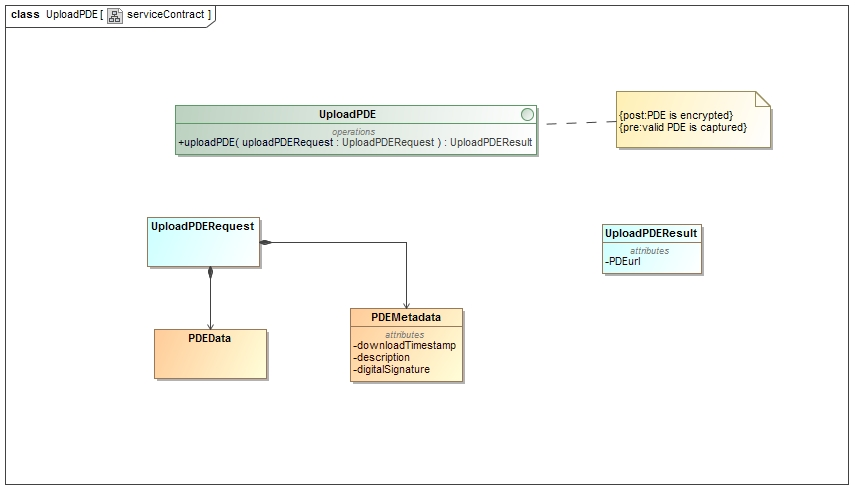
\includegraphics[width=\textwidth]{images/UploadserviceContract.jpg}
\caption{Service Contract: Uploading Potential Digital Evidence \label{overflow}}
\end{figure}\newpage
\textbf{Functional Requirement}\newline
A user needs to be able to upload a picture, video or audio.\newline
\begin{figure}[H]	
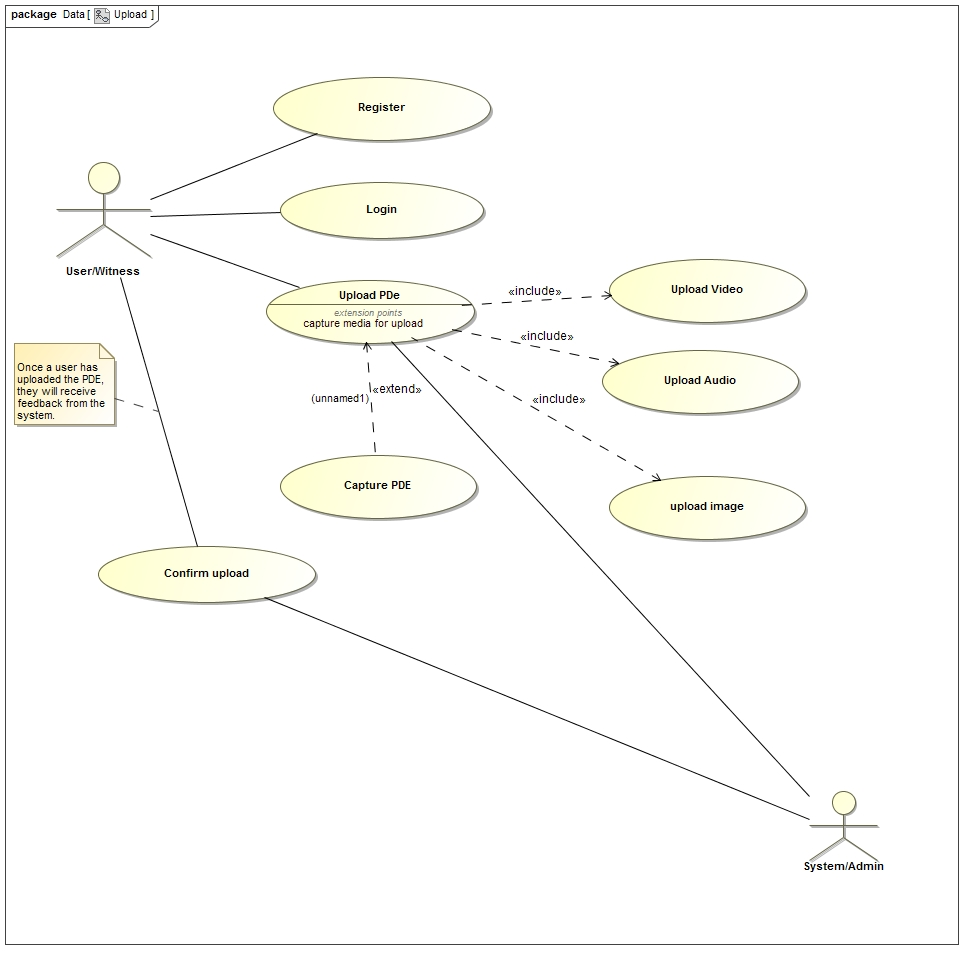
\includegraphics[width=\textwidth]{images/upload.jpg}
\caption{Functional Requirements: Uploading Potential Digital Evidence \label{overflow}}
\end{figure}
\begin{figure}[H]
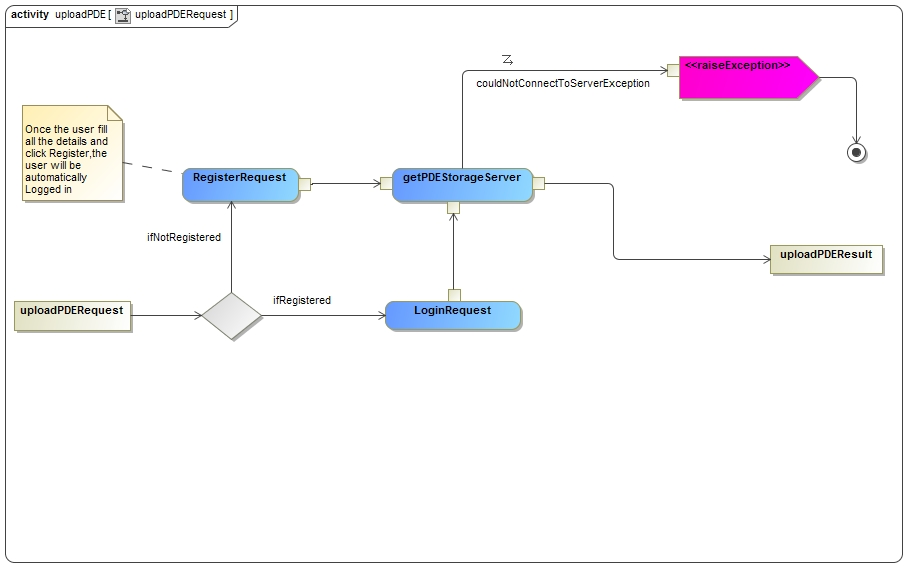
\includegraphics[width=\textwidth]{images/uploadPDERequest.jpg}
\caption{Process Specification: Uploading Potential Digital Evidence \label{overflow}}
\end{figure}
\subsubsection{ConfirmPDE-Priority:important}
\textbf{Service Contract}\newline
pre-condition: The user must have uploaded something to be confirmed.\newline
post-condition: The user gets a confirmation from the system.\newline
\textbf{Functional Requirement}\newline
The user waits to receive a confirmation from the system telling them if their PDE was accepted or rejected.\newpage
\subsection{The Administration Module}
The functionality provided by the Administration module includes the following:
\begin{itemize}
\item It manages access to the systems desktop version of the model
\item It provides means to download the potential digital evidence
\item It provides functionality to validate the evidence, whether by location, date and time or digital signature
\item It provides encryption and decrypt functionality
\end{itemize}
\subsubsection{DownloadPDE-Priority:critical}
\textbf{Service Contract}\newline
pre-condition: For any media to be downloaded, the media must be in the database.\newline
post-condition: The PDE must be persistent\newline
post-condition: The PDE is received\newline
\begin{figure}[H]
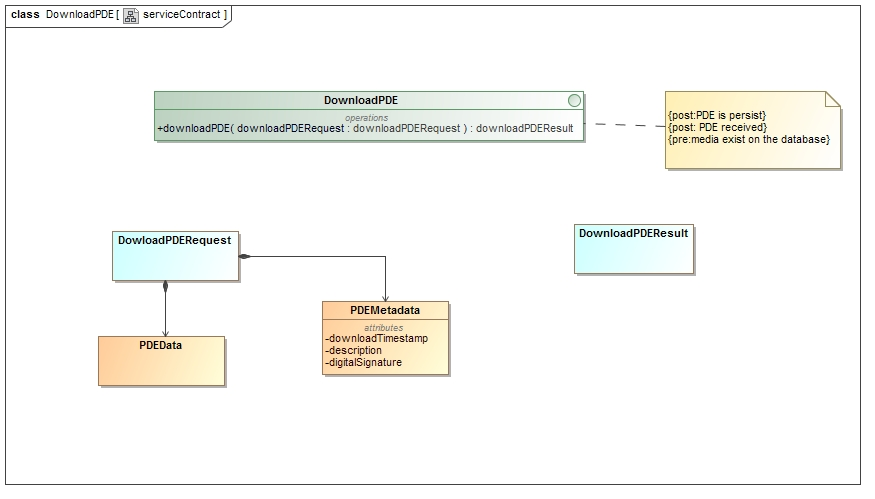
\includegraphics[width=1.0\textwidth]{images/downloadserviceContract.jpg}
\caption{Service Contract: Downloading Potential Digital Evidence \label{overflow}}
\end{figure}
\textbf{Functional Requirement}\newline
	The law enforcement agent needs to download the PDE to use it in the court of law. \newpage
\begin{figure}[H]
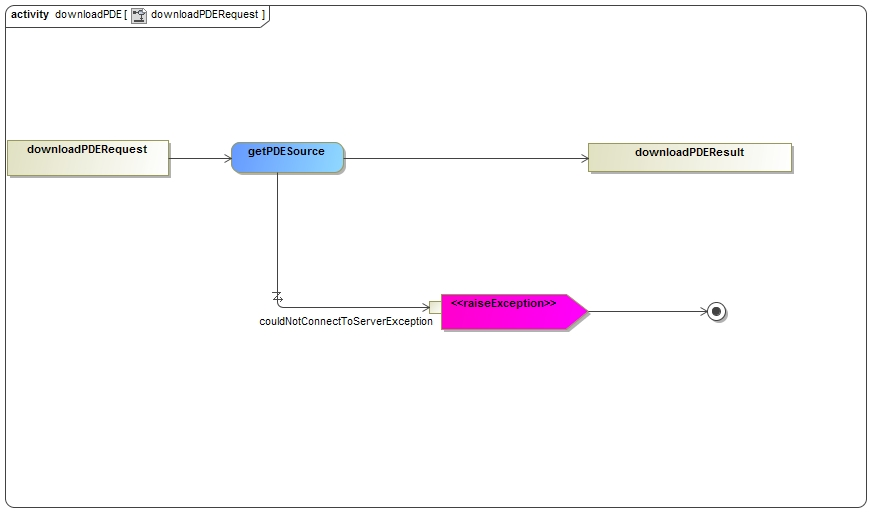
\includegraphics[width=\textwidth]{images/downloadPDERequest.jpg}
\caption{Process Specification: Downloading Potential Digital Evidence \label{overflow}}
\end{figure}	
\subsubsection{ValidatePDE-Priority:critical}
\textbf{Service Contract}\newline
post-condition: The PDE should be checked if it conforms to the standard set for valid evidence\newline
pre-condition: There has to be data to be validated\newline
\textbf{Functional Requirement}\newline
The system needs to validate that the data to ensure it's integrity.\newline
\subsubsection{EncryptPDE-Priority:critical}
\textbf{Service Contract}\newline
post-condition: The PDE should be encrypted.\newline
\textbf{Functional Requirement}\newline
	The system encrypts the PDE for it to be stored in the database.\newline
\subsubsection{DecryptPDE-Priority:critical}
\textbf{Service Contract}\newline
post-condition: The PDE should be decrypted before it is used in the court of law.\newline
\textbf{Functional Requirement}\newline
The system decrypts the PDE for it to be viewed in the court of law.\newline
\begin{figure}[H]
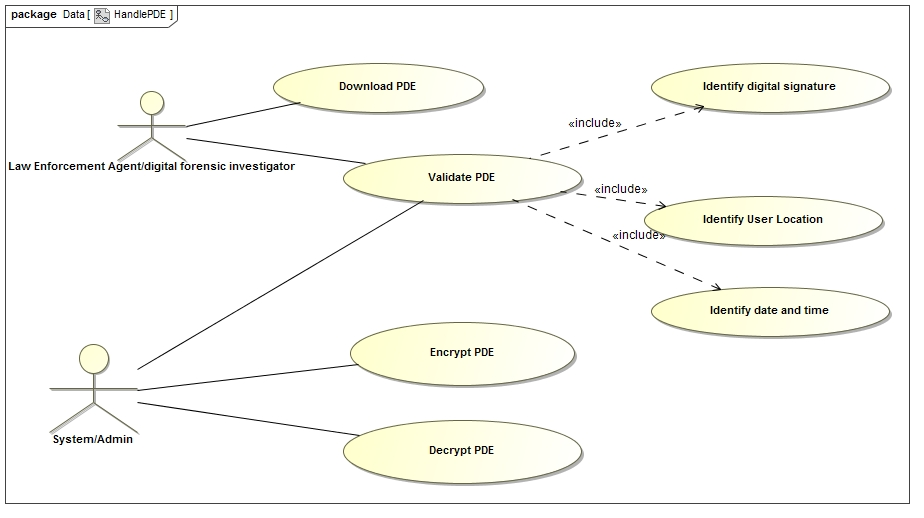
\includegraphics[width=\textwidth]{images/HandlePDE.jpg}
\caption{Functional Requirements: Validate,encrypt and decrypt PDE\label{overflow}}
\end{figure}
\subsubsection{ManageAccessAllocation-Priority:critical}
\textbf{Service Contract}\newline
post-condition: No unauthorised user can log in to the system.\newline
\textbf{Functional Requirement}\newline
The system is suppose to manage who has access to the system, this is a form of security measure.\newline
\begin{figure}[H]
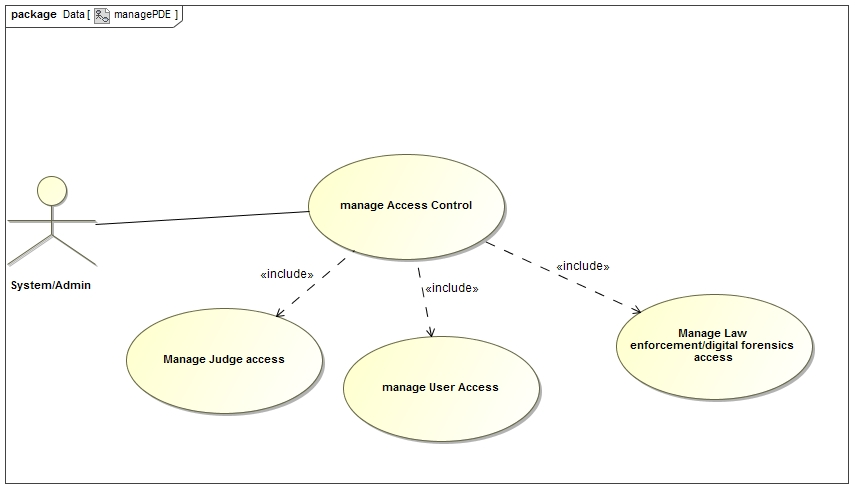
\includegraphics[width=\textwidth]{images/managePDE.jpg}
\caption{Functional Requirements: Manage Access Allocation\label{overflow}}
\end{figure}
\subsection{Login and Administrative user}
The system will authenticate against the South African Home Affairs Database for community members who are to upload potential digital evidence.\newline
The Login module provides services to login, view the potential digital evidence to be uploaded to the ONW system.\newline
\subsubsection{Login-Priority:critical}
\textbf{Service Contract}\newline
pre-condition: law enforcement agent and jury with provided credentials can login.\newline
pre-condition: Could connect to the SAPS database.\newline
post-condition: UserID on results is populated by user's ID.\newline
\begin{figure}[H]
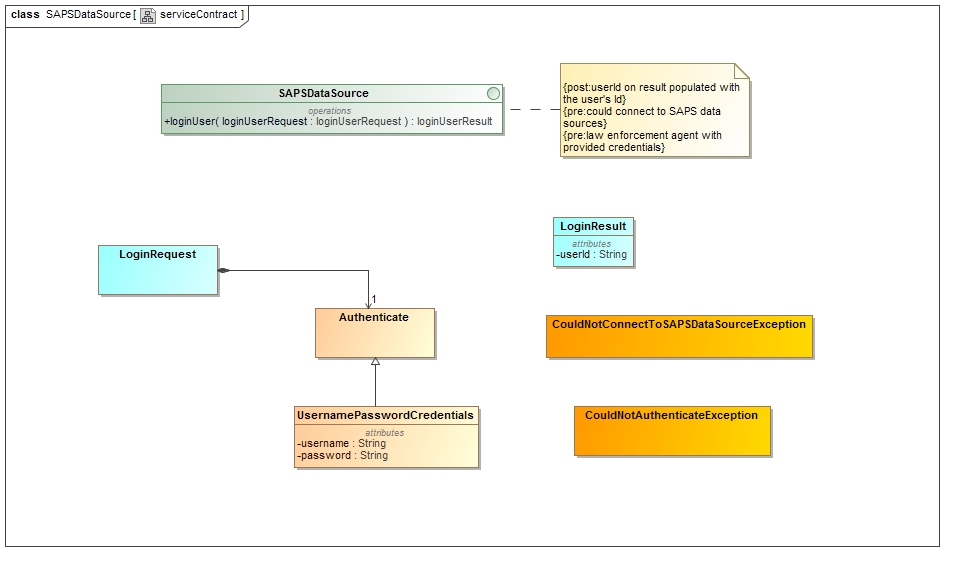
\includegraphics[width=\textwidth]{images/SAPSserviceContract.jpg}
\caption{Service Contract: Login for law enforcement and jury\label{overflow}}
\end{figure}\newpage
\textbf{Functional Requirement}\newline
The law enforcement agent should be able to log in to the system to view the PDE.\newline
\begin{figure}[H]
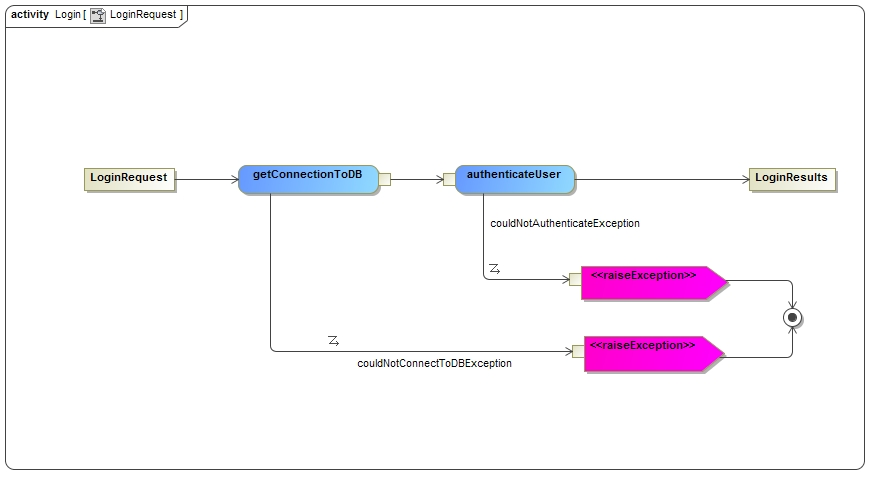
\includegraphics[width=\textwidth]{images/LoginRequest.jpg}
\caption{Process Specification: Login for law enforcement and jury\label{overflow}}
\end{figure}
\subsubsection{ViewPDE-Priority:important}
\textbf{Service Contract}\newline
pre-condition: The PDE is in the database to be viewed.\newline
post-condition: The law enforcement agent can view the PDE.\newline
\begin{figure}[H]
\includegraphics[width=\textwidth]{images/viewServiceContract.jpg}
\caption{Service Contract: View Potential Digital Evidence.\label{overflow}}
\end{figure}\newpage
\textbf{Functional Requirement}\newline
The law enforcement agents should be able to view what the witness has uploaded.\newline
\begin{figure}[H]
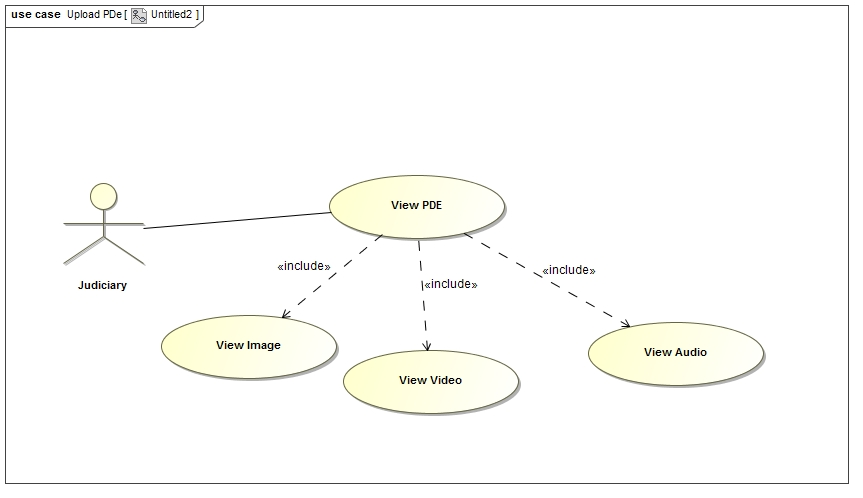
\includegraphics[width=\textwidth]{images/view.jpg}
\caption{Functional Requirements: View PDE\label{overflow}}
\end{figure}
\newpage
\subsection{Functionalities implemented}
Here are list of functionalities we have implemented from our system's use cases.
\begin{itemize}
	\item Geolocation: ability to detect the system's location at the time the evidence is captured.
	\item Detect internet connection: ability to tell whether there was internet connection when the evidence was captured.
	\item Capture PDE: ability to capture images, record audio and video as evidence with our system.
	\item Upload PDE: ability to send evidence to the database and retrieving it as needed.
	\item Tagging: ability for the law enforcement to search PDE file by tags.
	\item Download PDE: ability for the law enforcement to download pde.
	\item View PDE: ability for the users and law enforcement to view what has been uploaded
	\item Login and registration: ability for system users to login or register themselves in order to use the system.
	\item Access control: law enforcement and users have different rights levels
\end{itemize}

\newpage
\subsection{References}
\begin{itemize}
\item S.Omeleze,H.S.Venter, Toward a model for acquiring digital evidence using mobile devices. Information and Computer Security Architecture (ICSA) Research Group, University of Pretoria.
\item AGILE METHODOLOGY (author and date unknown)
	Available from: http://agilemethodology.org/ [Accessed: 15 May 2015]
\end{itemize}

\end{document}
